\documentclass{article}
\usepackage[utf8]{inputenc}
\usepackage{amsmath}
\usepackage{graphicx}

\title{Assinment 5}
\author{Swapnil Sirsat}
\date{January 2021}

\begin{document}

\maketitle

\section*{Question}
Construct a triangle $\Delta$PQR, PQ = 3, QR = 5.5 and $\angle$PQR = 60$^\circ$
\section*{Answer}
Given PQ = 3, QR = 5.5 and $\angle$PQR = 60$^\circ$ \\ 
now, \\
taking Q at (0,0)
equation of line PQ 
\begin{gather*}
    y = \sqrt{3}x
\end{gather*}
length of PQ = 3 \\
therefore the point ($x_1$,$y_1$) on line y =$\sqrt{3}$ x which is 3 units from (0,0)

\begin{gather*}
    \sqrt{x_1^{2}+y_1{2}} = 3 \\
    x_1^{2}+y_1{2} = 3^{2}\\
    x_1^{2}+3x_1^{2} = 9 \\
    4x_1^{2} = 9 \\
    x_1^{2} = \frac{9}{4}\\
    x_1 = 1.5\\
    \implies y = \sqrt{3} 1.5\\
\end{gather*}
therefore P(1.5,$\sqrt{3}1.5$), Q(0,0), R(5.5,0) are the point for the triangle PQR
\newpage
The following is the constructed figure
\begin{figure}[h!]
    \centering
    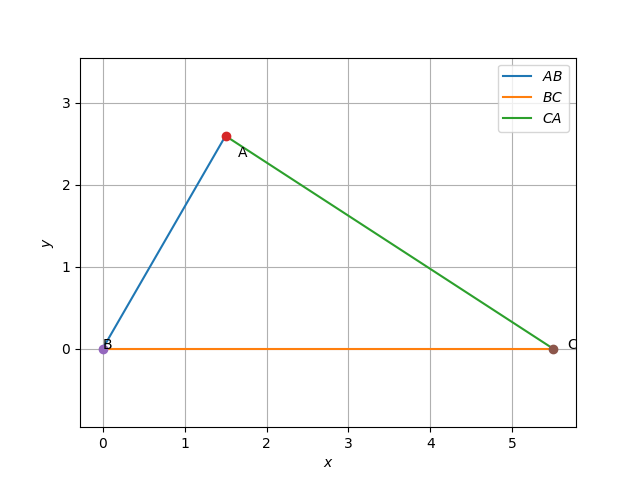
\includegraphics{Figure_1.png}
    \caption{Output of python code}
    \label{fig:my_label}
\end{figure}
\newpage
\newpage
\section{Question}
Construct $\Delta$ABC given that $\angle$A = 60$^\circ$, $\angle$B = 30$^\circ$ and AB = 5.8.
\section{Answer}
Given,
\begin{gather*}
    \angle A = 60^\circ \\
    \angle B = 30^\circ 
\end{gather*}
Now, by angle sum property
\begin{gather*}
    \angle A + \angle B + \angle C = 180^\circ \\
    \implies \angle C = 90^\circ
\end{gather*}
therefore $\Delta$ABC is a right angled triangle\\
Therefore, \\
\begin{gather*}
    \sin{A} = \frac{BC}{AB} = \frac{a}{5.8}\\
    \implies a = 5.8\sin{(60)}\\
    \implies a = 5.02\\
    \cos{A} = \frac{AC}{AB} = \frac{b}{5.8}\\
    \implies b = 5.8\cos{(60)} = 2.9
\end{gather*}
therefore 
\begin{gather*}
    a = 5.02\\
    b = 2.9 \\
    c = 5.8
\end{gather*}
\newpage
Below is the constructed figure
\begin{figure}[h!]
    \centering
    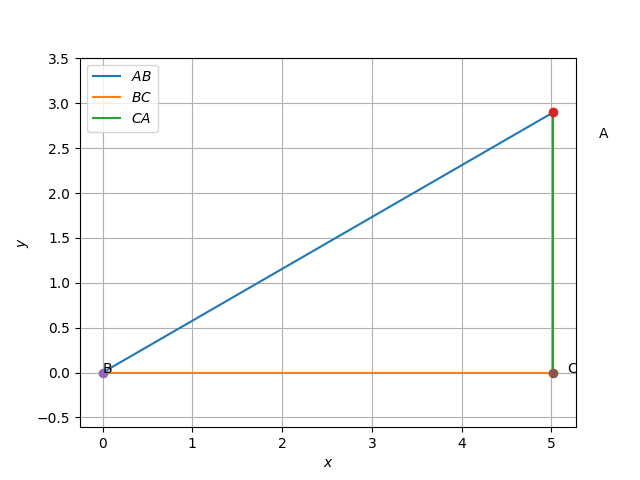
\includegraphics{Figure_2.png}
    \caption{Caption}
    \label{fig:my_label}
\end{figure}




\end{document}
